% \documentclass{article}
\documentclass[UTF8]{article}
% \usepackage{xeCJK}
\usepackage{ctex}
% if you need to pass options to natbib, use, e.g.:
%\PassOptionsToPackage{numbers, compress}{natbib}
% before loading nips_2017
%
% to avoid loading the natbib package, add option nonatbib:
% \usepackage[nonatbib]{nips_2017}

\usepackage[final]{nips_2017}

% to compile a camera-ready version, add the [final] option, e.g.:
% \usepackage[final]{nips_2017}

\usepackage[utf8]{inputenc} % allow utf-8 input
\usepackage[T1]{fontenc}    % use 8-bit T1 fonts
\DeclareRobustCommand\nobreakspace{\leavevmode\nobreak\ }
\usepackage{hyperref}       % hyperlinks
\usepackage{url}            % simple URL typesetting
\usepackage{booktabs}       % professional-quality tables
\usepackage{amsfonts}       % blackboard math symbols
\usepackage{nicefrac}       % compact symbols for 1/2, etc.
\usepackage{microtype}      % microtypography
\usepackage{bm}             % bold in math
\usepackage{graphicx}       % images
\usepackage{algorithm}      % algorithm
\usepackage[noend]{algpseudocode} % algorithm
\usepackage{caption}        % captionof
\usepackage{array}          % thick column hline
\usepackage{booktabs}       % table style
\usepackage{pbox}           % table line break
\usepackage{subcaption}     % multiple figures
\usepackage{listings}
\usepackage{xcolor}
\usepackage{tikz}
\usepackage{amsmath}
\definecolor{mygreen}{rgb}{0,0.6,0}
\definecolor{mygray}{rgb}{0.5,0.5,0.5}
\definecolor{mymauve}{rgb}{0.58,0,0.82}
\definecolor{codeBkg}{rgb}{0.85,0.85,0.85}

\lstset{
	backgroundcolor=\color{codeBkg},   % choose the background color; you must add \usepackage{color} or \usepackage{xcolor}; should come as last argument
	basicstyle=\footnotesize,        % the size of the fonts that are used for the code
	breakatwhitespace=false,         % sets if automatic breaks should only happen at whitespace
	breaklines=true,                 % sets automatic line breaking
	captionpos=b,                    % sets the caption-position to bottom
	commentstyle=\color{mygreen},    % comment style
	deletekeywords={...},            % if you want to delete keywords from the given language
	escapeinside={\%*}{*)},          % if you want to add LaTeX within your code
	extendedchars=true,              % lets you use non-ASCII characters; for 8-bits encodings only, does not work with UTF-8
	frame=no,	                   % adds a frame around the code
	keepspaces=true,                 % keeps spaces in text, useful for keeping indentation of code (possibly needs columns=flexible)
	keywordstyle=\color{blue},       % keyword style
	language=Octave,                 % the language of the code
	morekeywords={*,...},            % if you want to add more keywords to the set
	numbers=left,                    % where to put the line-numbers; possible values are (none, left, right)
	numbersep=5pt,                   % how far the line-numbers are from the code
	numberstyle=\tiny\color{mygray}, % the style that is used for the line-numbers
	rulecolor=\color{black},         % if not set, the frame-color may be changed on line-breaks within not-black text (e.g. comments (green here))
	showspaces=false,                % show spaces everywhere adding particular underscores; it overrides 'showstringspaces'
	showstringspaces=false,          % underline spaces within strings only
	showtabs=false,                  % show tabs within strings adding particular underscores
	stepnumber=1,                    % the step between two line-numbers. If it's 1, each line will be numbered
	stringstyle=\color{mymauve},     % string literal style
	tabsize=4,	                   % sets default tabsize to 2 spaces
	title=\lstname                  % show the filename of files included with \lstinputlisting; also try caption instead of title
}

\title{高级量化交易技术}

\hypersetup{
    colorlinks = true,
}
\makeatletter
% \def\BState{\State\hskip-\ALG@thistlm}
\def\BState{\hskip-\ALG@thistlm}
\makeatother
\floatname{algorithm}{Procedure}
\renewcommand{\algorithmicrequire}{\textbf{Input:}}
\renewcommand{\algorithmicensure}{\textbf{Output:}}

\newcolumntype{?}{!{\vrule width 3pt}}

\author{
  闫涛 \\
  %% examples of more authors
  %% \And
  %% Nicholas Frosst \\
  %% Affiliation \\
  %% Address \\
  %% \texttt{email} \\
  %% \AND
  %% Geoffrey E. Hinton \\
  科技有限公司\\
  北京 \\
  \texttt{\{yt7589\}@qq.com} \\
  %% Affiliation \\
  %% Address \\
  %% \texttt{email} \\
  %% \And
  %% Coauthor \\
  %% Affiliation \\
  %% Address \\
  %% \texttt{email} \\
  %% \And
  %% Coauthor \\
  %% Affiliation \\
  %% Address \\
  %% \texttt{email} \\
}
\date{Dec 2019}

% \usepackage{natbib}
% \usepackage{graphicx}

\begin{document}

\newpage
\maketitle
\begin{center}
\quad \newline \quad \newline \quad \newline \quad \newline \quad \newline \quad \newline \quad \newline \quad \newline \quad \newline \quad \newline
\quad \newline \quad \newline \quad \newline \quad \newline \quad \newline \quad \newline \quad \newline \quad \newline \quad \newline \quad \newline
\quad \newline \quad \newline \quad \newline \quad \newline \quad \newline \quad \newline \quad \newline \quad \newline \quad \newline \quad \newline
\quad \newline \quad \newline \quad \newline
\Large \textbf{第一篇 深度强化学习} \quad \textbf{}
\end{center}

\newpage
\maketitle
\begin{center}
\Large \textbf{第1章 强化学习概述} \quad 
\end{center}
\begin{abstract}
在本章中我们将讨论强化学习中的环境、Agent、状态、Action和奖励,并重点讨论MDP相关内容。
\end{abstract}
\section{MDP概述}
一个典型的强化学习系统结构如下所示:
\begin{figure}[H]
	\caption{典型强化学习系统架构图}
	\label{p000001}
	\centering
	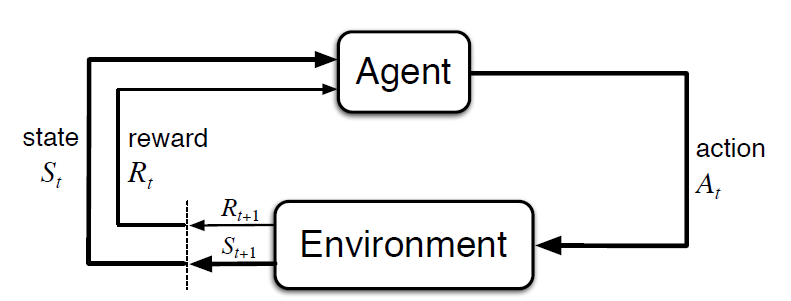
\includegraphics[width=15cm]{images/p000001}
\end{figure}
如图所示:
\begin{enumerate}
    \item 在$t$时刻Agent观察到环境状态$S_{t}$,并得到上一时刻所采取的行动$A_{t-1}$(在图中未画出)所得到的
奖励$r_{t}$;
    \item Agent根据环境状态$S_{t}$,根据某种策略$\pi$,选择行动$A_{t}$;
    \item 环境接收到Agent的行动$A_{t}$后,根据环境的动态特性,转移到新的状态$S_{t+1}$,并产生$R_{t}$的奖励
信号;
\end{enumerate}
\subsection{典型环境}
\subsubsection{Bandit Walk环境}
下面我们来研究一个最简单的强化学习环境,叫Bandit Walk,如下所示:
\begin{figure}[H]
	\caption{Bandit Walk环境图}
	\label{p000002}
	\centering
	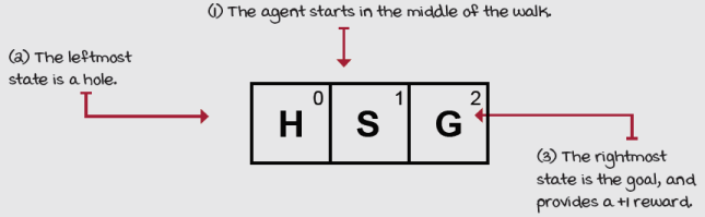
\includegraphics[width=15cm]{images/p000002}
\end{figure}
如图所示,Agent初始时位于中间的S格,状态编号为$S_{0}$,其可以采取向左、向右两个动作,向左则进入状态$H$,其是一个洞,就会掉到洞里,
过程就会结束,此时得到的奖励为0;当Agent采取向右行动时,就会进入G状态,此时会获得奖励+1,由此可见其是一个确定性的环境,就是说当
Agent采取向右行动时,会100\%确定进行G状态。我们可以通过如下的图来表示上述过程:
\begin{figure}[H]
	\caption{Bandit Walk环境MDP图}
	\label{p000003}
	\centering
	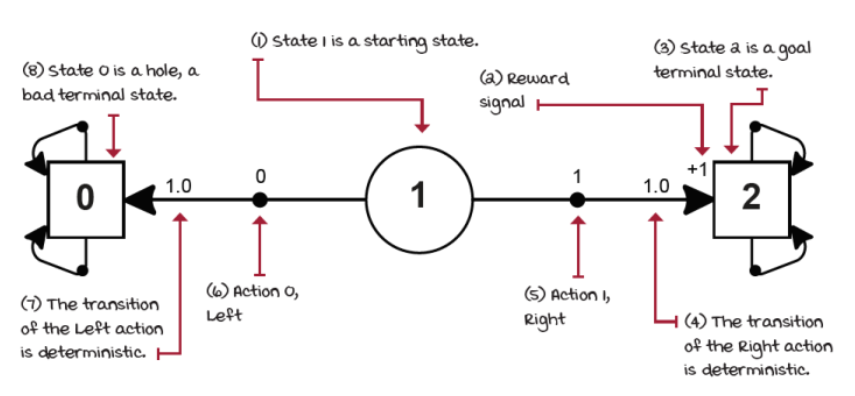
\includegraphics[width=15cm]{images/p000003}
\end{figure}
如图所示:
\begin{itemize}
    \item 在初始状态$S_{0}$时,有两个可选行动,分别表示为向左、向右的直线;
    \item 当采取向右行动时,就会到达小黑点位置,然后由环境决定将转到哪个状态,以及转到这个状态的概率,以本例为例,其就是以100\%
的概率转到G状态$S_{2}$,其中小黑点上面的1代表行动编号,向右简头上面的1.0代表100\%的概率,向右简头处的1代表奖励为+1;
\end{itemize}
我们首先安装所需要的库:
\lstset{language=PYTHON, caption={安装gmy库}, label={pip-install-gym}}
\begin{lstlisting}
pip install gym -i https://pypi.tuna.tsinghua.edu.cn/simple 
\end{lstlisting}
下面我们用Python对象来表示这一过程:
\lstset{language=PYTHON, caption={Bandit Walk python程序}, label={bandit-walk-python-env}}
\begin{lstlisting}
P = {
    0: {
        0: [(1.0, 0, 0.0, True)],
        1: [(1.0, 0, 0.0, True)]
    },
    1: {
        0: [(1.0, 0, 0.0, True)],
        1: [(1.0, 2, 1.0, True)]
    },
    2: {
        0: [(1.0, 2, 0.0, True)],
        1: [(1.0, 2, 0.0, True)]
    }
}
print(P)
\end{lstlisting}
代码解读如下所示:
\begin{itemize}
    \item P为一个字典对象,其键值0、1、2代表三个状态;
    \item P的键值0:其同样是一个字典对象,键值代表可以采取的行动,0代表向右,1代表向右;
    \item P的键值0下键值0:即在状态0下面采取行动0,其值为一个数组,代表由环境决定要转到哪个状态,转到每个状态为一个Turple,含
义为:(概率, 目的状态,获得奖励,新状态是否为终止状态),注意:我们规定在终止状态采取任何行动都会回到自身;
\end{itemize}
上面我们仅举了一个例子,其他状态读者可以自己解析出来。
\subsubsection{Bandit Slippery Walk环境}
在上面的环境中,我们向左移动,环境会确定地向左移动。但是在本节中,当我们向左移动时,环境在80\%的情况下会向左移动,20\%的情况会
向右移动。如下图所示:
\begin{figure}[H]
	\caption{Bandit Slippery Walk环境图}
	\label{p000004}
	\centering
	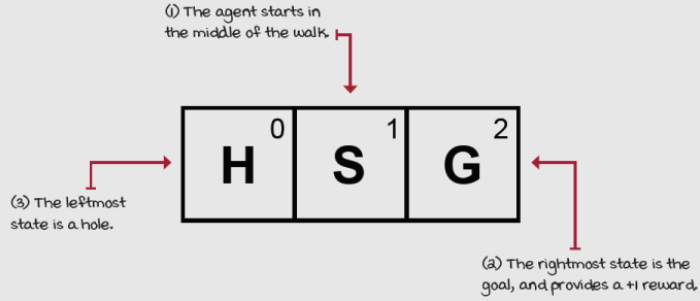
\includegraphics[width=15cm]{images/p000004}
\end{figure}
除了环境的随机性之外,环境与上一节相同。其MDP图如下所示:
\begin{figure}[H]
	\caption{Bandit Slippery Walk环境MDP图}
	\label{p000005}
	\centering
	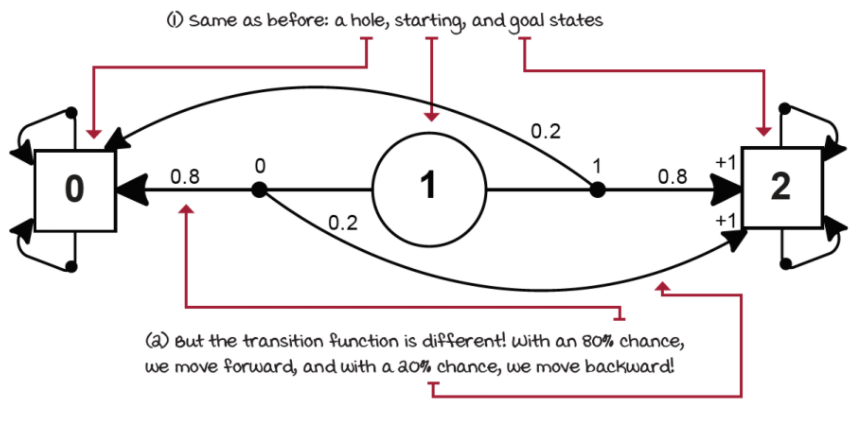
\includegraphics[width=15cm]{images/p000005}
\end{figure}
如上图所示,在开始时Agent位于状态S,其可以采取的行动为向左编号为0或向右编号为1,我们以向右为例,当Agent采取向右行动时,其达到状态S右侧的小黑点,上面的1代表是编号为1的行动,
此时环境将以80\%的概率转变为状态G,得到+1的奖励,如图中的右箭头所示,同时环境还可能将以20\%的概率变为状态H,其所获得的奖励为0,如图中向左的曲线箭头所示。读者可以按照上面
的描述,自己补充出其他状态变化情况。由前面的讨论可以看出,在这个例子中,当Agent采取向右行动Action时,环境仅以80\%的概率完成该Action,同时还可能以20\%的概率向相反的方向
变化,既环境具有一定的随机性。
我们可以通过如下的Python代码来表示这一过程:
\lstset{language=PYTHON, caption={Bandit Slippery Walk python程序}, label={bandit-slippery-walk-python-env}}
\begin{lstlisting}
    def bandit_slippery_walk(self):
        P = {
            0: {
                0: [(1.0, 0, 0.0, True)],
                1: [(1.0, 0, 0.0, True)]
            },
            1: {
                0: [(0.8, 0, 0.0, True), (0.2, 2, 1.0, True)],
                1: [(0.8, 2, 1.0, True), (0.2, 0, 0.0, True)]
            },
            2: {
                0: [(1.0, 2, 0.0, True)],
                1: [(1.0, 2, 0.0, True)]
            }
        }
        print(P)
\end{lstlisting}
如上所示,在状态S时,如果采取编号为0的向左行动,则有80\%的概率会进入到状态H,奖励为0.0,并且是终止状态,当采用编号为1的向右行动时,将进入状态G,获得奖励为1.0,并且为终止状态,
采用这种方式我们就表示了环境的随机性。
\subsection{典型交互}
Agent与环境的交互分为分段的或连续的,由一系列时间步聚组成,在时间$t$时刻:
\begin{itemize}
    \item Agent得到环境给的奖励信号$R_{t}$,其由Agent在上一时刻$S_{t-1}$采取行动$A_{t-1}$时所获得的,并且Agent观察到环境状态$S_{t}$;
    \item Agent根据所观察到的环境状态$S_{t}$,选择采取行动$A_{t}$;
    \item 环境接收到行动$A_{t}$后,会转移到新的状态$S_{t+1}$,并且会给Agent奖励$R_{t+1}$;
    \item 依次循环......
\end{itemize}
上述过程可以表示为:
\begin{equation}
\begin{aligned}
(R_{0}, S_{0}, A_{0}), (R_{1}, S_{1}, A_{1}), (R_{2}, S_{2}, A_{2}), ..., (R_{t}, S_{t}, A_{t}), ..., (R_{T}, S_{T}, A_{T})
\end{aligned}
\label{mdp-episode-trajectory}
\end{equation}
\subsection{MDP定义}
我们以Frozen Lake为例来定义MDP过程。该环境如下所示:
\begin{figure}[H]
	\caption{Frozen Lake环境图}
	\label{p000006}
	\centering
	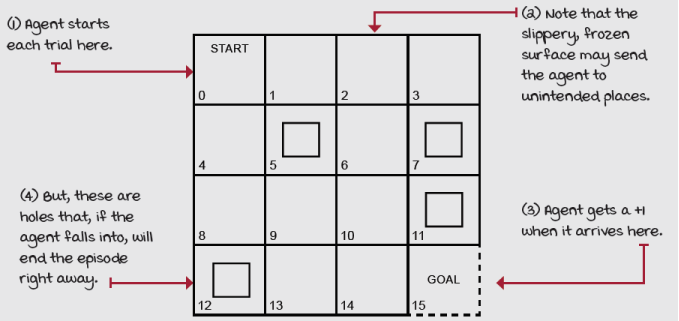
\includegraphics[width=15cm]{images/p000006}
\end{figure}
如图所示:
\begin{itemize}
    \item Agent从状态Start开始;
    \item 在每个状态,Agent可以采取向左、向上、向下、向右行动,当在边缘状态时,走出环境的行动会100\%使Agent留在原状态;
    \item 由于是冻冰的湖面,例如当Agent选择向下行动时,其有33.3\%的概率向下运动,还有66.7\%的概率会向垂直的方向运动,既以33.3\%的概率向左运动,33.3\%的概率向右运动;
    \item 当Agent到达有洞的状态时,过程立即结束;
    \item 当Agent到达最终节点时,可以获得+1的奖励;
\end{itemize}
\subsubsection{环境状态建模}
时刻$t$环境状态的状态表示为$S_{t}$,环境所有可能的状态用集合$\mathcal{S}$表示,通常我们用$n$维向量来表示一个状态:
\begin{equation}
\begin{aligned}
S_{t}=\boldsymbol{s} = \begin{bmatrix}
    s_{1} \\
    s_{2} \\
    ... \\
    s_{n}
\end{bmatrix} \in R^{n}
\end{aligned}
\label{state-vector-representation}
\end{equation}
对于我们当前研究的这个问题,环境状态只需要表示Agent处于哪个状态即可,我们采用0$\sim$15来对状态进行编号,因此状态可以用0$\sim$15来表示:
\begin{equation}
\begin{aligned}
S_{t}=\boldsymbol{s} = \begin{bmatrix}
    i
\end{bmatrix} \in R^{1}, i \in \{0, 1, 2, 3, ..., 15\}
\end{aligned}
\label{frozen-lake-state-demo}
\end{equation}
我们规定环境只与当前状态有关,而与过去的历史无关,这就是马可夫特性,即我们研究的过程是无记忆的。乍一看,这是一个非常严重的限制条件,但是在实际应用中,我们通常可以通过设计合适的状态,使
所研究的问题变为无记忆的。用数学语言可以表示为:
\begin{equation}
\begin{aligned}
P(S_{t+1} | S_{t}, A_{t}) = P(S_{t+1} | S_{t}, A_{t}, S_{t-1}, A_{t-1}, ...)
\end{aligned}
\label{markov-property-def}
\end{equation}
以Frozen Lake为例,其每个状态和在状态上可以采取的行动如下所示:
\begin{figure}[H]
	\caption{Frozen Lake状态和行动图}
	\label{p000007}
	\centering
	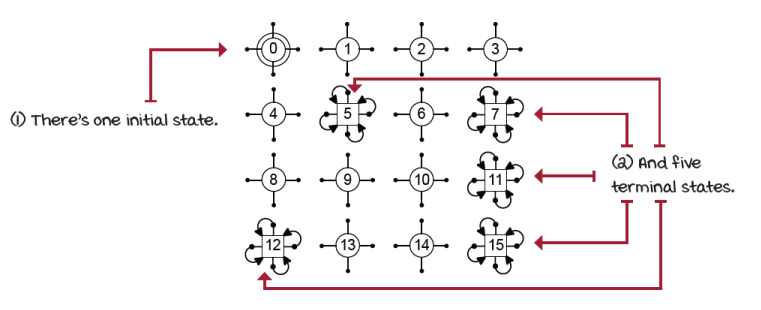
\includegraphics[width=15cm]{images/p000007}
\end{figure}
当Ageng采取行动后,环境会根据自身的动态特性,转移到下一个状态,我们称之为转移函数,如下图所示:
\begin{figure}[H]
	\caption{Frozen Lake状态转移图}
	\label{p000008}
	\centering
	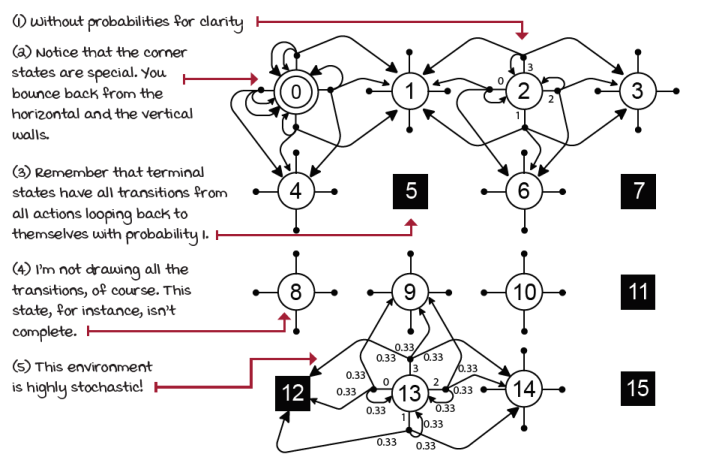
\includegraphics[width=15cm]{images/p000008}
\end{figure}
在状态13时,共有向左、向下、向右、向上编号分别为0、1、2、3的四种行动,当Agent采取行动0向左时,将到达左侧的小黑点,
\begin{itemize}
    \item 行动0(向左):到达左侧小黑点,由于冻冰原因,其有如下三种可能性:
    \begin{itemize}
        \item 33.3\%:向左,进入状态12,获取奖励0.0,并且为终止状态,用(0.333, 12, 0.0, True)表示;
        \item 33.3\%:向下,由于是边缘节点,其仍然在状态13,获取奖励0.0,不为终止状态,用(0.333, 13, 0.0, False)表示;
        \item 33.3\%:向上,进入状态9,获取奖励为0.0,不是终止状态,用(0.33, 9, 0.0, False)表示;
    \end{itemize}
    \item 行动1(向下):到达下面小黑点,有如下三种可能性:
    \begin{itemize}
        \item 33.3\%(向下):由于是边缘节点,其仍然在状态13,获得奖励为0.0,不是终止状态,用(0.333, 13, 0.0, False)表示;
        \item 33.3\%(向左):进入状态12,获得奖励0.0,并且为终止状态,用(0.333, 12, 0.0, True)表示;
        \item 33.3\%(向右):进入状态14,获得奖励0.0,不是终止状态,用(0.333, 14, 0.0, False)表示;
    \end{itemize}
\end{itemize}
我们这里仅举了两个例子,其余内容读者可以自己补全。
环境的状态转移函数如下所示:
\begin{equation}
\begin{aligned}
p(s' | s, a) = P(S_{t}=s' | S_{t-1}=s, A_{t-1}=a) \\
\sum_{s' \in S} p(s' | s, a) = 1, \forall s \in S, \forall a \in A(s)
\end{aligned}
\label{env-state-transition-function}
\end{equation}
上式表明在任意时刻,环境状态为$S_{t-1}=s$,Agnet采取行动为$A_{t-1}=a$时,环境由于具有随机性,以一个确定的概率分布进入新状态$S_{t}=s'$,并且
如果我们将所有可能到达的新状态的概率相加,其值为1。
当Agent根据自己的策略,在任意时刻采取行动后,系统会给Agent一个奖励Reward,其是一个标量,越大代表该行动决策越好,越小代表越差,甚至可以为负值,代表需要尽力避免
的情况。需要注意的是,Agent不仅要关注当前获得的奖励,还要关注最终获得的累积的奖励,Agent的目标就是使最终获得的累积奖励最大。
环境的奖励函数如下表示:
\begin{equation}
\begin{aligned}
r(s, a) = E\bigg( R_{t} | S_{t-1}=s, A_{t-1}=a \bigg)
\end{aligned}
\label{env-reward-function}
\end{equation}
上式表明在$t-1$时刻,环境状态为$S_{t-1}=s$,Agent采取行动$A_{t-1}=a$,环境在$t$时刻给出奖励$R_{t}$,由于环境具有随机性,环境可能进入不同的状态,从而获得不同的奖励,
而且即使是进入同一个状态,获得的奖励也有可能不同,因此在这种情况,下的奖励就是所有这种情况下获得奖励的期望值。
在$t-1$时刻,环境状态为$S_{t-1}=s$,Agent采取行动$A_{t-1}=a$,环境进入$S_{t}=s'$时,获得的奖励为:
\begin{equation}
\begin{aligned}
r(s, a, s') = E\bigg( R_{t} | S_{t-1}=s, A_{t-1}=a, S_{t}=s' \bigg)
\end{aligned}
\label{env-reward-function-sas}
\end{equation}
从上式就可以看出,即使是转移到同一个状态,也可能获得不同的奖励,所以我们将奖励定义所有这些值的期望。
在上面我们定义在任意时刻,Agent通过与环境交互,获得的奖励为$R_{t}$,同时我们知道,Agent的目标是使整个过程,所有时刻所获得奖励的累加值最大,我们将其定义为回报$G_{t}$。但是由于未来具有更大的不确定性,
因此距离当前时间点越近,获得的奖励就越有价值,越远则价值越小,因此我们引入折扣的概念,如下所示:
\begin{equation}
\begin{aligned}
G_{t} = R_{t+1} + \gamma R_{t+2} + \gamma ^{2} R_{t+3} + ... + \gamma ^{k-1} R_{t+k} + ... + R_{T} \\
= \sum_{k=0}^{\infty} \gamma ^{k} R_{t+k+1} \\
=R_{t+1} + \gamma G_{t+1}
\end{aligned}
\label{env-reward-function-sas}
\end{equation}

\subsection{状态值函数}
我们假定Agent的策略为$\pi$,我们定义当Agent在某个状态可以获得的累积奖励的期望值为该状态的值函数,如下所示:
\begin{equation}
\begin{aligned}
v_{\pi}(s) = E_{\pi}(G_{t} | S_{t}=s) = E_{\pi} (R_{t+1} + \gamma G_{t+1} | S_{t}=s)
\end{aligned}
\label{state-value-function-definition}
\end{equation}
由于上式是求期望值,根据期望值定义,可以得到:
\begin{equation}
\begin{aligned}
v_{\pi}(s) = \sum_{a} \pi (a|s) \sum_{s', r} p(s', r | s, a) (r + \gamma v_{\pi}(s'))
\end{aligned}
\label{state-value-function-definition}
\end{equation}

\newpage
\maketitle
\begin{center}
\quad \newline \quad \newline \quad \newline \quad \newline \quad \newline \quad \newline \quad \newline \quad \newline \quad \newline \quad \newline
\Large \textbf{第二篇 时序信号分析} \quad \textbf{}
\end{center}




\newpage
\maketitle
\begin{center}
\quad \newline \quad \newline \quad \newline \quad \newline \quad \newline \quad \newline \quad \newline \quad \newline \quad \newline \quad \newline
\Large \textbf{第三篇 量化交易平台} \quad \textbf{}
\end{center}


\newpage
\maketitle
\begin{center}
\quad \newline \quad \newline \quad \newline \quad \newline \quad \newline \quad \newline \quad \newline \quad \newline \quad \newline \quad \newline
\Large \textbf{第四篇 50ETF期权} \quad \textbf{}
\end{center}


\newpage
\maketitle
\begin{center}
\quad \newline \quad \newline \quad \newline \quad \newline \quad \newline \quad \newline \quad \newline \quad \newline \quad \newline \quad \newline
\Large \textbf{第五篇 50ETF量化交易} \quad \textbf{}
\end{center}



\section{附录X}

\newpage

\bibliographystyle{plainnat}
\bibliography{nips}

\appendix

\end{document}



